\documentclass[t,aspectratio=169]{beamer}
%\usepackage{fale}

%%% presentation below

\title{Ansible}
\subtitle{Configuration Management System done right}
\author{Fabio Alessandro Locati}
\date{25 October 2016}

\begin{document}

\maketitle

\begin{frame}
    \frametitle{Outline}
    \tableofcontents
\end{frame}

\section{Intro}
\begin{frame}
    \frametitle{About me}
    \begin{itemize}
        \item<2-> IT Consultant since 2004
        \item<3-> Ansible user since 2013
    \end{itemize}
\end{frame}

\begin{frame}
    \frametitle{Idempotence}
    \begin{definition}{Idempotence}
    is the property of certain operations in mathematics and computer science, that can be applied multiple times without changing the result beyond the initial application. 
    \end{definition}
\end{frame}

\begin{frame}
    \frametitle{Ansible}
    \begin{itemize}
        \item<2-> Written in Python
        \item<3-> Mainly push mode
        \item<4-> Advantages
        \begin{itemize}
            \item<5-> Infrastructure as \textbf{Data} (in YAML format)
            \item<6-> Very gentle learning curve
            \item<7-> Very simple setup
            \item<8-> Balanced tool
        \end{itemize}
        \item<9-> Disadvantages
        \begin{itemize}
            \item<10-> Not very good introspection tools
            \item<11-> Community is young
        \end{itemize}
    \end{itemize}
\end{frame}

\section{Ansible}
\begin{frame}
    \frametitle{Ansible concepts}
    \begin{itemize}
        \item<2->\textbf{Host}: Target of the execution
        \item<3->\textbf{Module}: Modules can control system resources, like services, packages, or files (anything really), or handle executing system commands.
        \item<4->\textbf{Module library}: Default set of modules coming with Ansible basic installation
        \item<5->\textbf{Task}: An istance of a Module 
        \item<6->\textbf{Role}: A way to abstract a collection of tasks that has a specific role and is idempotent
        \item<7->\textbf{Playbook}: A collection of Tasks and Roles that could be idempotent (or not)
    \end{itemize}
\end{frame}

\begin{frame}[fragile]
    \frametitle{Ansible infrastructure}
    \begin{semiverbatim}
+---------------------+
|     GIT Server      |
+---------------------+     .
           |                .
           |                .   +---------------------+
           V                |-->|   Controlled Host   |
+---------------------+     |   +---------------------+
| Ansible Controller  |-----|
+---------------------+     |   +---------------------+
                            |-->|   Controlled Host   |
                            .   +---------------------+
                            .
                            .
    \end{semiverbatim}
\end{frame}

\begin{frame}
    \frametitle{Layout}
    \begin{center}
        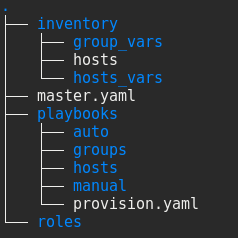
\includegraphics[scale=0.5]{project_structure.png}
    \end{center}
\end{frame}

\begin{frame}
    \frametitle{Links}
    \begin{itemize}
        \item Official documentation: http://docs.ansible.com
        \item Videos: https://www.ansible.com/videos
        \item Ebooks: https://www.ansible.com/ebooks
        \item Fedora Infrastructure: https://infrastructure.fedoraproject.org/cgit/ansible.git
        \item Ceph: https://github.com/ceph/ceph-ansible
        \item OpenStack: https://github.com/openstack/openstack-ansible
        \item OpenShift: https://github.com/openshift/openshift-ansible
    \end{itemize}
\end{frame}

%\makethanks

\end{document}
